\chapter{Projecte de sensors}
En aquest capítol es realitzarà un escenari real on s'implementarà la tecnologia BLE per transmetre dades.
Primerament es realitzaran proves per veure les capacitats del protocol i de la placa que s'esta utilitzant.

\section{Experimentació}
Per comprendre millor com afecten els diferents paràmetres configurables corresponents a BLE i també les prestacions dels perifèrics de la placa es realitzaran els següents escenaris.


\subsection{Abast}

Com s'ha mencionat anteriorment l'abast teòric que té BLE és considerable comparat amb les tecnologies similars.
Però cal entendre que al estar utilitzant la banda de 2.4 GHz, l'abast de BLE dependrà de l'entorn, on pot haver-hi molta variabilitat d'interferències.
És per això que en un escenari realista l'abast que es pot assolir pot ser molt diferent del teòric.
Les LAUNCHXL-CC1352R1 utilitzades per a aquest treball, per si soles, no són l'eina perfecte per fer proves d'abast.
Això es deu, en part, a que no es pot transmetre a la màxima potència permesa per l'estàndard que és de fins a 20 dBm.
Com a molt es pot transmetre a 5 dBm i per defecte només s'utilitzen 0 dBm de potència en transmissió.
Per realitzar un experiment que fos més precís seria avantatjós utilitzar una antena externa més directiva.
Enlloc d'analitzar l'abast de la tecnologia en aquest apartat es farà un balanç comparatiu per veure les diferències reals d'utilitzar les diferents capes físiques de BLE.

Per a aquest apartat es va realitzar un experiment pràctic en un lloc relativament aïllat i on es pogués tenir una suficient distància amb visibilitat directa.
Es va escollir un pàrquing i es va utilitzar la potència per defecte de 0 dBm per poder treballar amb distàncies més curtes.

\begin{figure}[!h]
	\begin{center}
		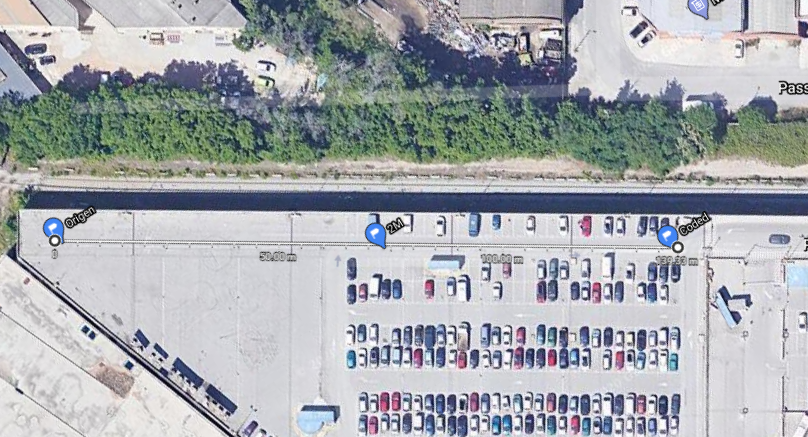
\includegraphics[width=\textwidth]{./images/prova_abast.png}
		\caption{Abast}
	\end{center}
\end{figure}

El procediment per realitzar l'experiment va ser deixar una de les plaques sobre un cotxe i amb l'altre connectada a una altre ordinador anar retrocedint fins que es perdés la connexió.
Per forçar que es perdés la connexió quan ja no es podia establir una comunicació des de la placa que s'anava movent s'anaven enviant peticions de lectura d'atributs.

El resultat va ser d'una distància màxima de 75 metres amb la capa física de 2M i de 135 metres quan s'utilitzava la capa Coded S=8.
S'analitzarant només aquestes capes físiques ja que al no haver-hi interferències significants i sempre es mantenia visibilitat directe els resultats de la capa 1M eren similars als de 2M i els de Coded S=2 eren similar als de S=8.

Amb aquest experiment s'ha validat tal i com s'havia comentat anteriorment els avantatges que aporta la nova capa física Coded que no existia abans de la versió 5.0 de BLE.
Amb aquest rang en visibilitat directe es pot considerar que BLE podrà assolir cobertura suficient dins les cases a través de parets.

En aquest apartat només s'ha vist una de les millores de la capa física Coded però també cal recordar que on també és extremadament útil a part de l'abast és en el de resistència a les interferències.
Aquest component seria interessant poder-lo provar en un futur (queda per fer).


\subsection{Consum d'Energia}

El consum dels dispositius que utilitzen BLE és molt important ja que aquesta tecnologia està dissenyada per a consumir la menor quantitat d'energia possible.
Les plaques utilitzades tenen ponts extraïbles que permeten desconnectar els components que no son essencials per al funcionament del xip CC1352.
D'aquesta manera es pot utilitzar un analitzador de potència per mesurar l'energia consumida pel xip.
Amb aquesta configuració es pot tenir una mesura molt precisa i poder calcular el cicle de vida del dispositiu que s'està desenvolupant.
Però aquesta configuració no permet utilitzar les eines de desenvolupament com la depuració del codi.

\begin{figure}[h]
	\begin{center}
		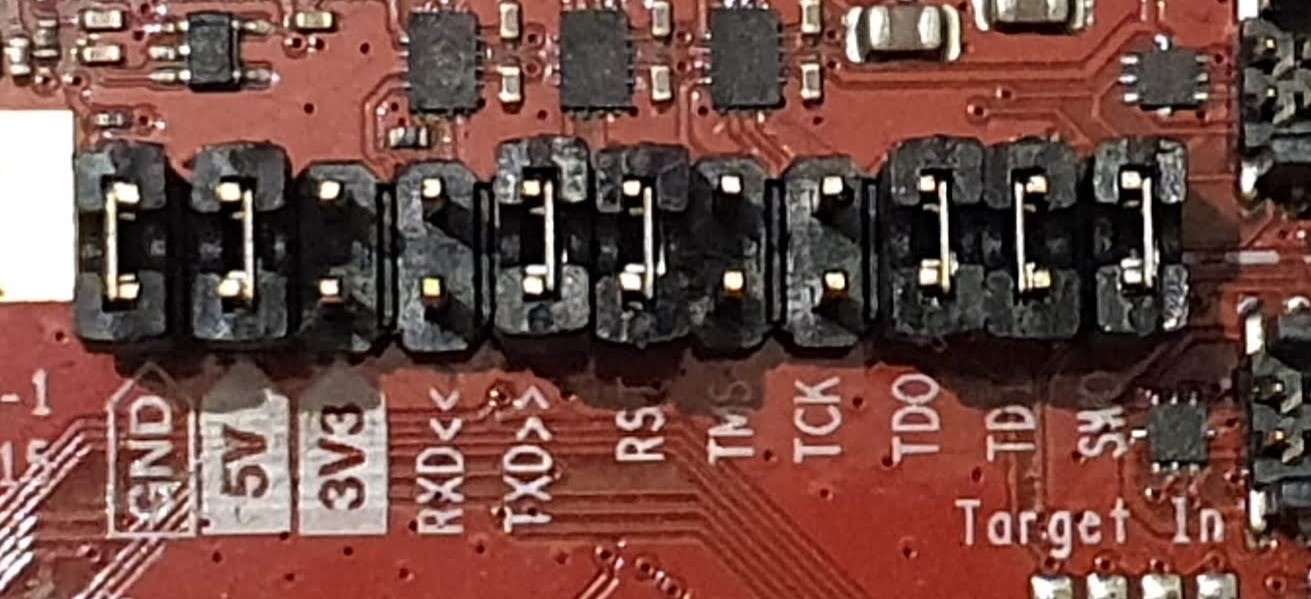
\includegraphics[width=0.7\textwidth]{./images/ponts.jpg}
		\caption{Ponts extraïbles de la placa}
	\end{center}
\end{figure}

Per poder fàcilment desenvolupar un projecte i analitzar els canvis que el codi produeix en l'ús d'energia hi ha una eina anomenada Energy Trace.
D'aquesta manera es pot analitzar comparativament en quin moment s'està consumint l'energia i es poden adaptar els paràmetres de la connexió per veure quin serà l'estalvi que s'aconseguirà.
Així es poden prendre les decisions de quins sacrificis es poden suportar pel que fa a latència, per exemple, a canvi de reduir el consum.
Aquesta eina però no substitueix la solució explicada anteriorment amb el analitzador de potència ja que l'Energy Trace resulta molt menys precisa.

Per veure un exemple de com funciona l'EnergyTrace s'ha utilitzat mentre el Project Zero s'estava executant al processador. A continuació es pot veure una captura d'un segon de duració del consum aproximat de corrent.
\begin{figure}[!h]
	\begin{center}
		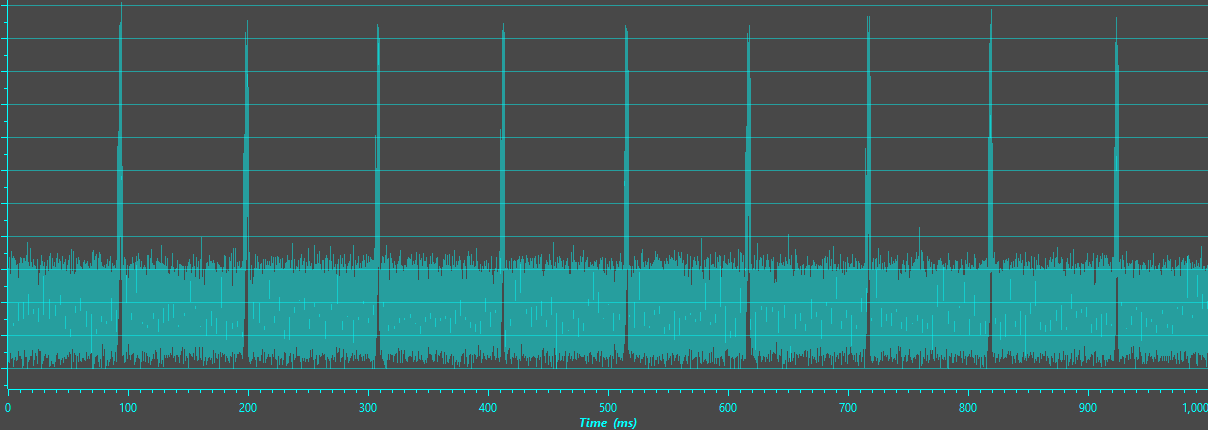
\includegraphics[width=\textwidth]{./images/energy_trace.png}
		\caption{Captura d'Energy Trace}
	\end{center}
\end{figure}

Es pot veure com hi ha pics de consum cada 100 ms, aquests corresponen als instants en que el dispositiu està enviant els anuncis.
El temps de 100 ms correspon al interval d'anunci que s'ha configurat per a aquest projecte.

Un cop s'estableix una connexió amb el dispositiu es torna a fer una altre captura d'un segon que es pot veure a continuació.

\begin{figure}[!h]
	\begin{center}
		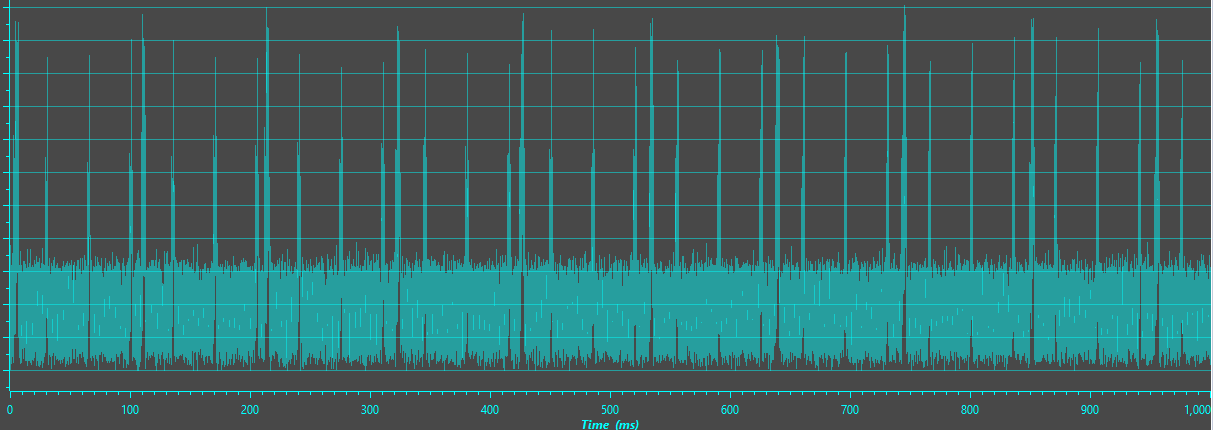
\includegraphics[width=\textwidth]{./images/energy_trace_2.png}
		\caption{Captura d'Energy Trace 2}
	\end{center}
\end{figure}

En aquesta captura es pot veure com segueixen estant els pics cada 100 ms però també n'hi ha cada 40 ms.
Aquests es deuen als esdeveniments de connexió que en aquest cas estan configurats per a que es produeixen cada 40 ms.

Aquesta eina per tant està orientada a tenir una idea comparativa de en quins instants es consumeix més energia.
D'aquesta manera és més fàcil pel desenvolupador prova canvis en el codi i veure com aquests afecten al consum d'energia.

%\section{Mesures Biològiques}

%Si es volen transmetre la velocitat dels batecs del cor això suposa, aproximadament, una mostra cada segon d'uns 10 bits més un instant de temps de 30 bits suposa uns 40 bits/segon, insignificant.

%Si el que es vol es transmetre el senyal directament que prové del sensor que mesura la sang.
%Considerem el màxim de 200 batecs per minut, això és una freqüència de 3,3 Hz, si mostregem a 10 vegades Fmax, 33 mostres/segon amb una resolució de 10 bits la tassa es de 330 bits/s

\subsection{Simulador de sensors}
La placa té un convertidor analògic-digital que ens permetrà enviar senyals analògiques un cop s'han mostrejat.
En aquest treball no es tractaran directament els sensors sinó que es simularan le senyals que en sortirien.
Com que la placa i el seu ADC treballa a 3.3V es crearà un circuit que permeti controlar un voltatge d'entre 0 i 3.3V.

Aquest circuit es basarà en un divisor de voltatge simple format per una resistència i un potenciòmetre.
El potenciòmetre permet canviar la resistència del element a través d'un cargol i junt amb el circuit que l'envolta permetrà canviar el voltatge a la sortida.
\begin{figure}[!h]
	\begin{center}
		\begin{circuitikz}
			\draw
			(0,2) node[anchor=east] {$V_{in}$}
			to [R=$R_1$, *-] (2,2)
			to [vR=$R_{pot}$, *-] (2,0) node[tlground](GND){};
			\draw
			(2,2) to [short, -*] (3,2)
			to (3,2) node[anchor=west] (3,2) {$V_{out}$};
		\end{circuitikz}
		
	\end{center}
\end{figure}

Aquest circuit segueix la estructura d'un divisor de voltatge per tant es pot calcular el voltatge a la sortida segons la següent fórmula.

\begin{equation}
	V_{in}\cdot\frac{R_{pot}}{R_1+R_{pot}}=V_{out}
\end{equation}

Per escollir els components cal tenir in compte utilitzar resistències de valor alt per reduir el consum d'energia.
S'utilitzarà un potenciòmetre de 10KOhms per tant serà una resistència que es podrà modificar des de 0 Ohms fins 10 KOhms.
Per trobar la $R_1$ que compleixi els requisits queda la següent fórmula.

\begin{equation}
	R_1=5V\cdot\frac{10k\Omega}{3.3V}-10k\Omega\approx5151\Omega
\end{equation}

Per a la $R_1$ s'utilitzaran resistències de la sèrie E12, els valors que més s'acosten a $5121\Omega$ són $5.6k\Omega$ i $4.6k\Omega$.
Per assegurar-se que no es superen els 3.3V a la entrada del ADC que podria malmetre el dispositiu s'escull la resistència superior, per tant el circuit final quedarà de la següent manera.

\begin{figure}[!h]
	\begin{center}
		\begin{circuitikz}
			\draw
			(0,2) node[anchor=east] {$5\,V$}
			to [R=$5.6\;k\Omega$, *-] (2,2)
			to [vR=$ \lbrack 0-10 \rbrack \;k\Omega$, *-] (2,0) node[tlground](GND){};
			\draw
			(2,2) to [short, -*] (3,2)
			to (3,2) node[anchor=west] (3,2) {$[0-3.3]\;V$};
		\end{circuitikz}
		
	\end{center}
\end{figure}

Com que s'utilitzaran 4 canals del ADC per prendre mesures es necessiten 4 circuits com el que s'ha dissenyat.
S'ha fet el circuit en una protoboard i soldat els components de tal manera que cal connectar el voltatge d'entrada (a 5V) en vermell, terra en negre i finalment quatre cables blaus on hi haurà el voltatge controlat pels quatre potenciòmetres.
A continuació es pot veure com ha quedat el circuit.

\begin{figure}[!h]
	\begin{center}
		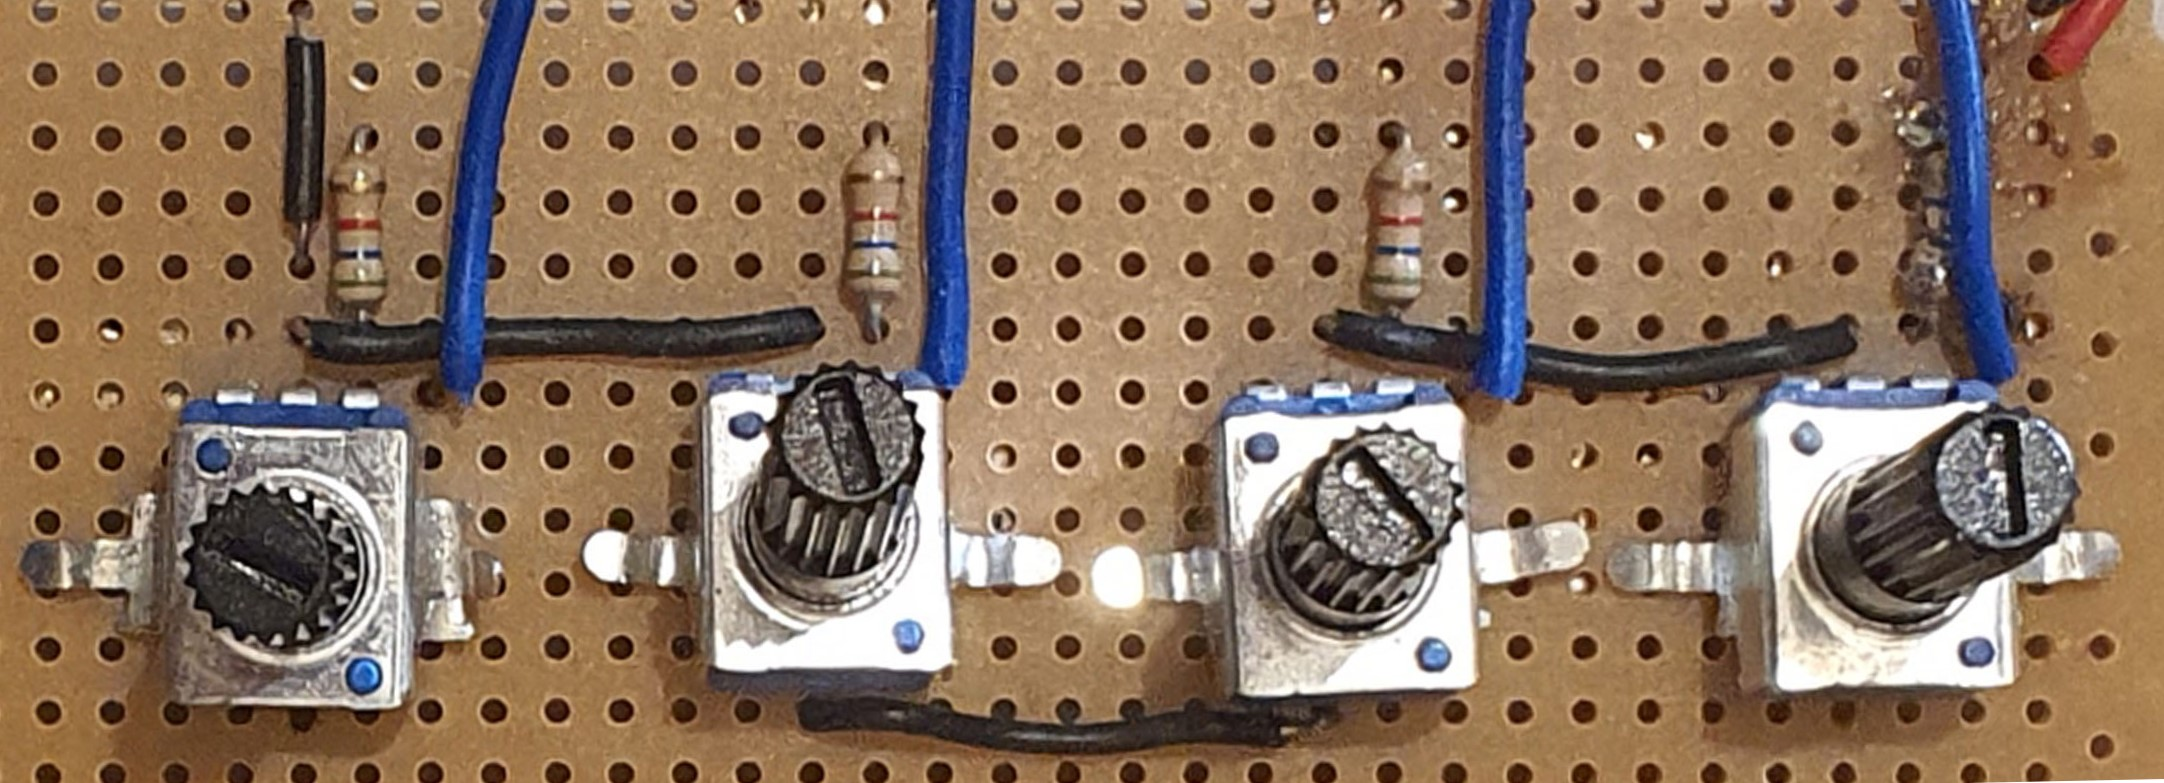
\includegraphics[width=0.6\textwidth]{./images/sensors_circuit.jpg}
		\caption{Circuit soldat}
	\end{center}
\end{figure}


\section{Lectura del ADC}
Tal i com s'ha comentat anteriorment la placa que estem utilitzant te un ADC que utilitzarem per llegir valors de voltatge.

%Importar adcsinglechannel
En aquest exemple l'objectiu es aconseguir poder llegir els valors del voltatge d'un pin de la placa.
El següent codi ens permet fer una mesura del canal que s'indiqui a través del argument i ens retorna el resultat en miliVolts.

%TODO: Pretify code
\begin{lstlisting}[language=C]
static uint16_t takeMeasurement(uint_least8_t adcIndex){
	ADC_Handle adc;
	ADC_Params params;
	ADC_init();
	ADC_Params_init(&params);
	adc = ADC_open(adcIndex, &params);
	if (adc == NULL){
		Log_info0("ADC start Failed");
		while(1);
	}
	int_fast16_t res;
	uint16_t adcValue;
	res = ADC_convert(adc, &adcValue);
	
	if (res == ADC_STATUS_SUCCESS) {
		Log_info1("ADC result %d mV", adcValue);
	}
	else {
		Log_info0("ADC status failure");
	}
	ADC_close(adc);
	return adcValue;
}
\end{lstlisting}

Finalment cal vanviar el codi de BLE per a que quan es llegeixin els atributs es retorni el valor mesurat al ADC.
Per tant cal canviar la funció environmentalService\_ReadAttrCB tal i com es veu a continuació.

\begin{lstlisting}[language=C]
  if(!memcmp(pAttr->type.uuid, temperatureUUID, pAttr->type.len))
{
	uint16_t adcValue = takeMeasurement(Board_ADC0);
	*pLen = (uint16_t)temperatureLen;
	memcpy(pValue, &adcValue, *pLen);
}
else if(!memcmp(pAttr->type.uuid, humidityUUID, pAttr->type.len))
{
	uint16_t adcValue = takeMeasurement(Board_ADC1);
	*pLen = (uint16_t)humidityLen;
	memcpy(pValue, &adcValue, *pLen);
}
\end{lstlisting}

\section{Aplicació mòbil}
Per veure un exemple simplificat d'un client que consumis els serveis oferits per la placa s'ha desenvolupat una aplicació per a Android.
Aquesta aplicació llegeix continuament els valors dels quatre atributs que té la placa relacionas amb el sensors.
El codi de la app es pot trobar a \cite{android_repo}.

Per poder interactuar amb la placa el primer que cal és tenir en compte l'adreça del dispositiu i els identificadors, tant del servei, com dels atributs. 

\begin{table}[!h]
	\begin{center}
		\begin{tabular}{|c|l|}
			\hline
			Identificador	&	Valor	\\	\hline
			deviceAddress	&	00:81:F9:4A:4D:B3	\\	\hline
			serviceUUID		&	f0001234-0451-4000-b000-00000000		\\	\hline
			temperatureUUID	&	f0002345-0451-4000-b000-000000000000	\\	\hline
			humidityUUID	&	f0003456-0451-4000-b000-000000000000	\\	\hline
			heartRateUUID	&	f0004567-0451-4000-b000-000000000000	\\	\hline
			bloodOxygenUUID	&	f0005678-0451-4000-b000-000000000000	\\	\hline
		\end{tabular}
	\end{center}
	\caption{Tipus d'anunciaments}
\end{table}

Les dades que s'estan transmetent per cada atribut corresponen al valor del voltatge.
Tot i així, per caracteritzar aquestes dades a l'aplicació s'interpreten com si fossin valors plausibles de les mesures que s'estan prenent.
Igualment, es mostra tant una barra de progrés com el valor real de milivolts per cada mesura de la placa.
A continuació es pot veura una captura de la applicació en funcionament.

\begin{figure}[h]
	\begin{center}
		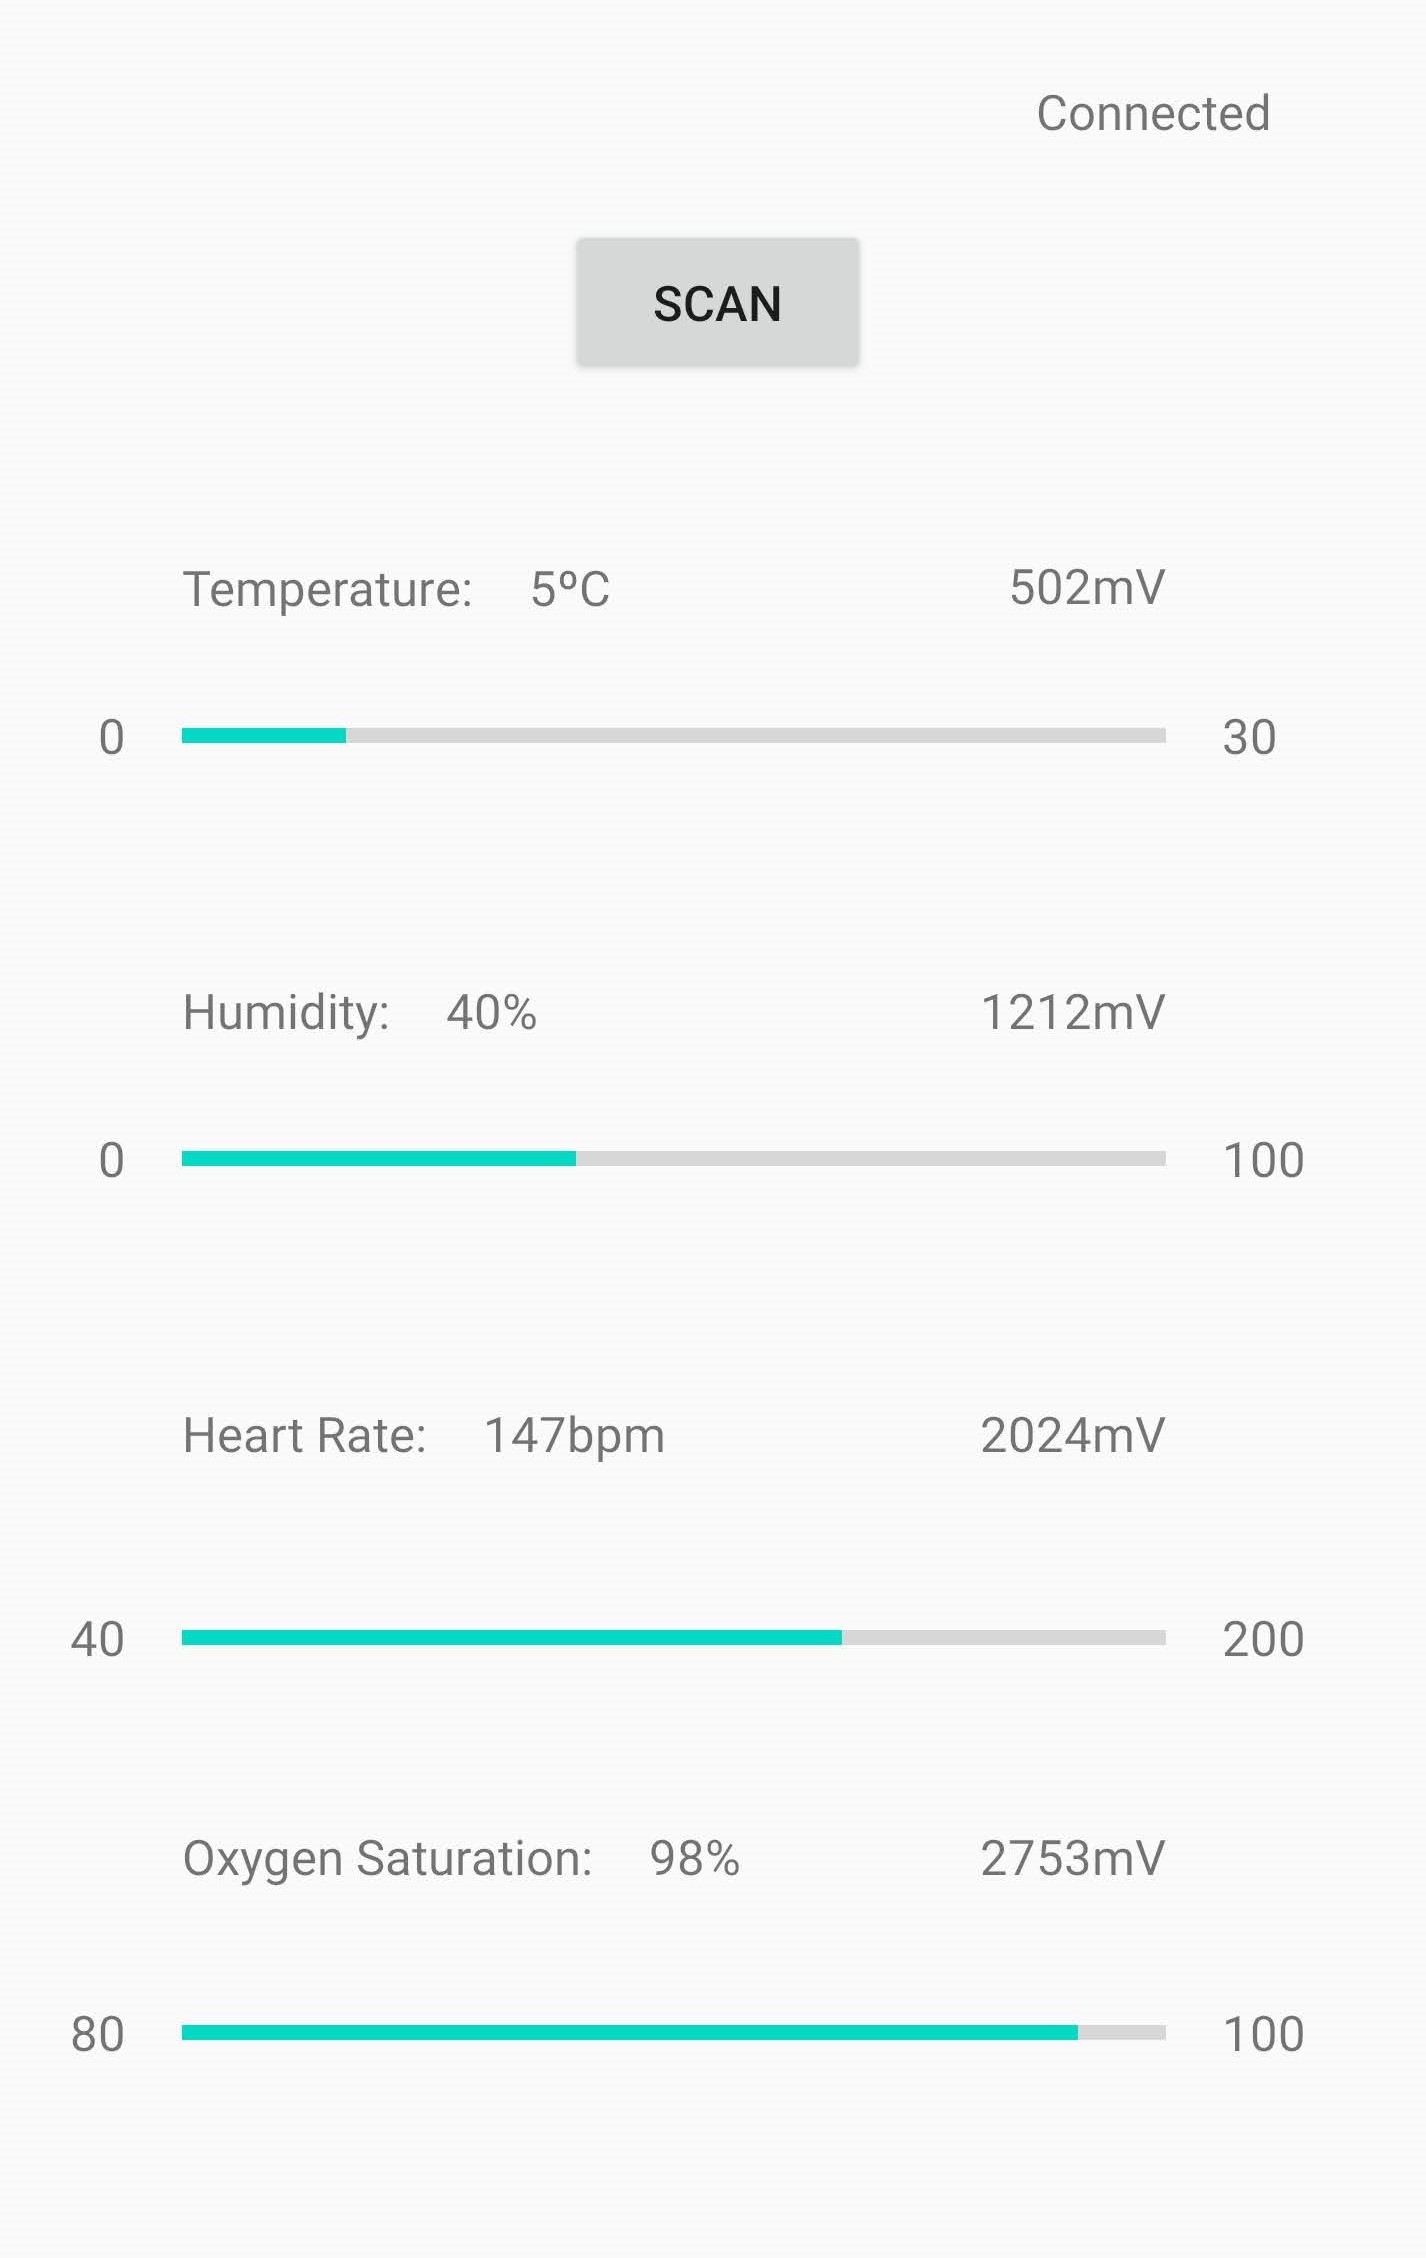
\includegraphics[width=0.4\textwidth]{./images/captura_app.jpg}
		\caption{Ports placa}
	\end{center}
\end{figure}

\section{Escenari}
Finalment, un cop desenvolupat el circuit per simular sensors, el codi necessari per mostrejar i transmetre els valors i una aplicació per rebre aquests valors, l'escenari és el següent.

El circuit que simula els 4 sensors es connecta als pins de la placa que tenen ADC segons el manual de la placa que es pot trobar a \cite{manual_placa}.
Segueixen aquesta taula:

\begin{table}[!h]
	\begin{center}
		\begin{tabular}{|c|c|c|}
			\hline
			ADC			&	DIO		& 	PIN		\\	\hline
			0			&	23		&	2		\\	\hline
			1			&	24		&	6		\\	\hline
			2			&	25		&	23		\\	\hline
			3			&	26		&	24		\\	\hline
		\end{tabular}
	\end{center}
	\caption{Taula dels pins amb ADC}
\end{table}

Per fer les connexions fins des del circuit fins la placa es fa a través dels ports que proporciona la placa a la seva part de darrera.

\begin{figure}[!h]
	\begin{center}
		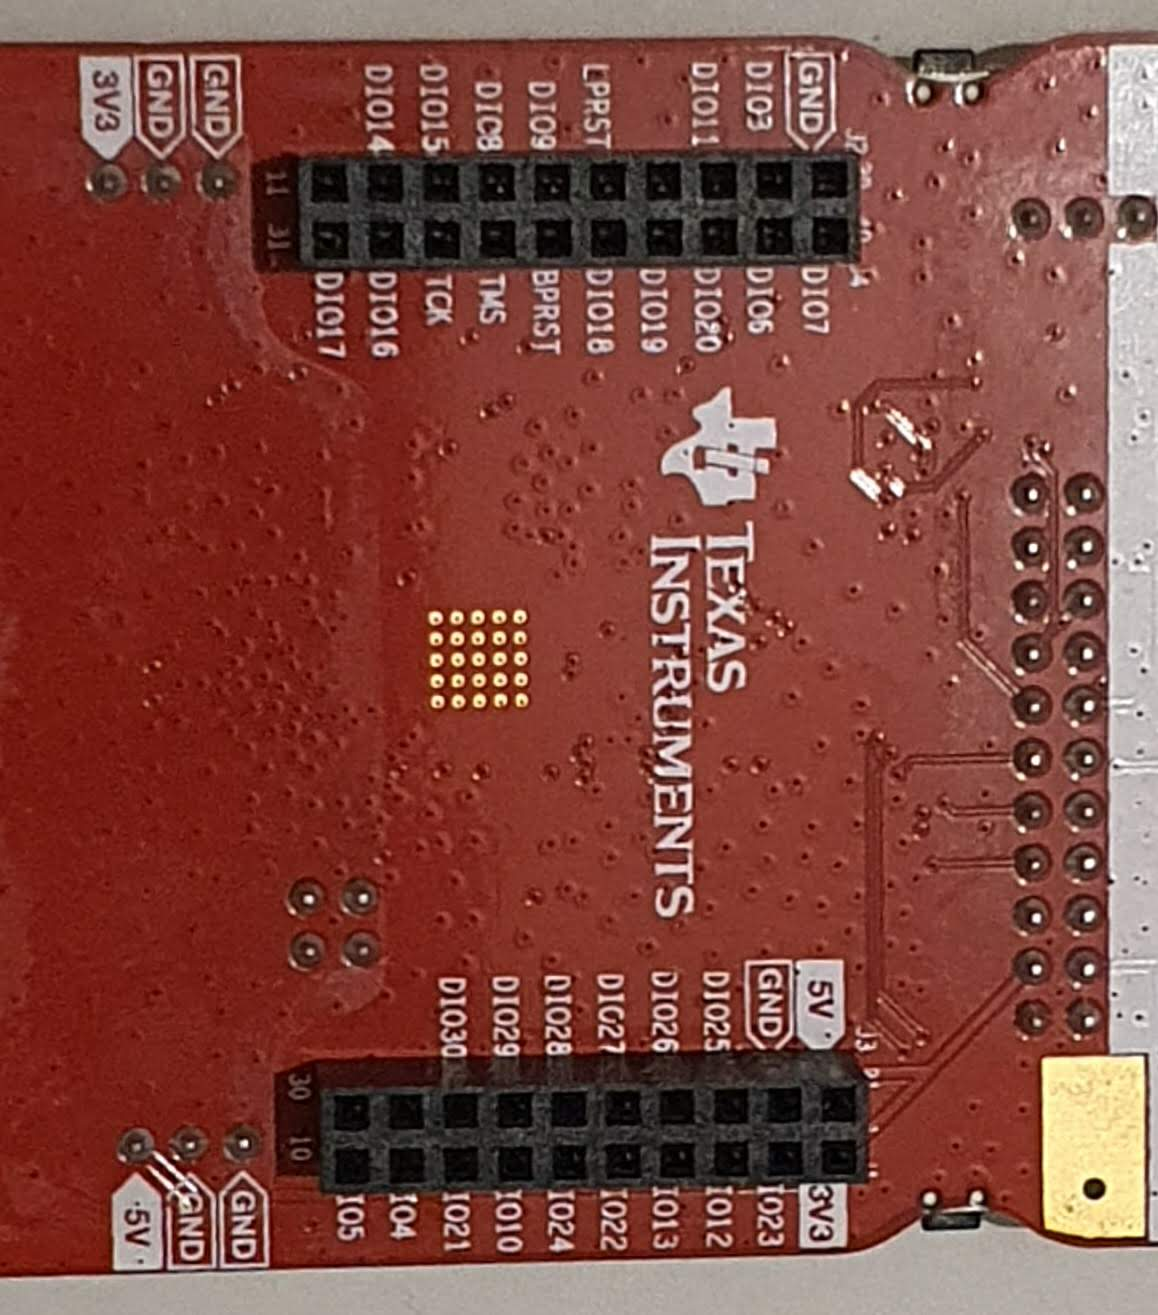
\includegraphics[angle=90, width=0.6\textwidth]{./images/connexions_placa.jpg}
		\caption{Ports placa}
	\end{center}
\end{figure}

Un cop les conexions estan fetes cal executar el codi de la placa i clicar el botó d'escanejar de l'aplicació.
Cal tenir en compte que durant el proces de d'escaneig degut a la configuració de BLE sempre és possible (tot i que poc probable) que el mòbil no descobreixi la placa un cop transcorregut el temps establert.
En cas que sigui així cal tornar a clicar el botó d'escaneig.
Un cop l'aplicació està ecanejant es poden canviar les posicions dels potenciòmetres i es veu com els valors corresponents en el mòbil canvien amb poca latència.

\section{Continuitat del treball}
Un cop realitzat el treball i entès tant el Bluetooth Low Energy com l'entorn de desenvolupament hi ha aspectes en que es podria entrar més en profunditat en cas que algú seguís amb aquest projecte tal i com he fet jo.

Tal i com s'ha esmentant quant s'ha realitzat l'estudi del consum d'energia utilitzant Energy Trace, els valors obtinguts no es poden considerar absoluts.
És per això que per poder determinar el temps de vida amb diferents configuracions del BLE s'hauria de mesurar el consum amb un oscil·loscopi mentre la placa esta configurada amb la font d'alimentació externa.

La implementació pràctica de BLE que s'ha realitzat no utilitza cap servei propietari.
Seria interessant implementar un servei estandaritzat i tenir algun dispositiu comercial que pogués connectar-se a la placa.

Finalment tot i haver-se desenvolupats projectes que permeten mesurar els voltatges dels ADCs i emetre notificacions per part de BLE, no s'ha aconseguit que sigui alhora.

